\chapter{Обзор литературы}

Внутренние волны очень распространенное явление в океане\cite{holton_encyclopedia_2003}. Существуют они благодаря перепадам плотности на разной глубине, сила плавучести играет роль восстанавливающей силы \cite{Eckart1961}. Океаны являются одним из естественных примеров стратифицированных сред. Основные источники внутренних волн в океане это приливные эффекты, которые сопряжены с движением Земли относительно Солнца и Луны относительно Земли \cite{Egbert2000}.

\section{История развития интереса к явлению внутренних волн и текущее состояние}

Считается установленным, что впервые внутренние волны наблюдал американский ученый Франклин в восемнадцатом веке с помощью простой экспериментальной установки. Она представляла собой емкость, заполненную несмешивающимися жидкостями различной полости~\cite{Sudolski}. Однако в конце восемнадцатого века вблизи полуострова Таймыр произошло событие, которое заострило внимание научного сообщества на этом интересном явлении. В то время в этом районе пролегал маршрут исследовательского судна <<Фрам>>(Рис. \ref{fig:fram}) под руководством Фритьофа Нансена (Рис. \ref{fig:Nansen}).

\begin{figure}
    \centering
    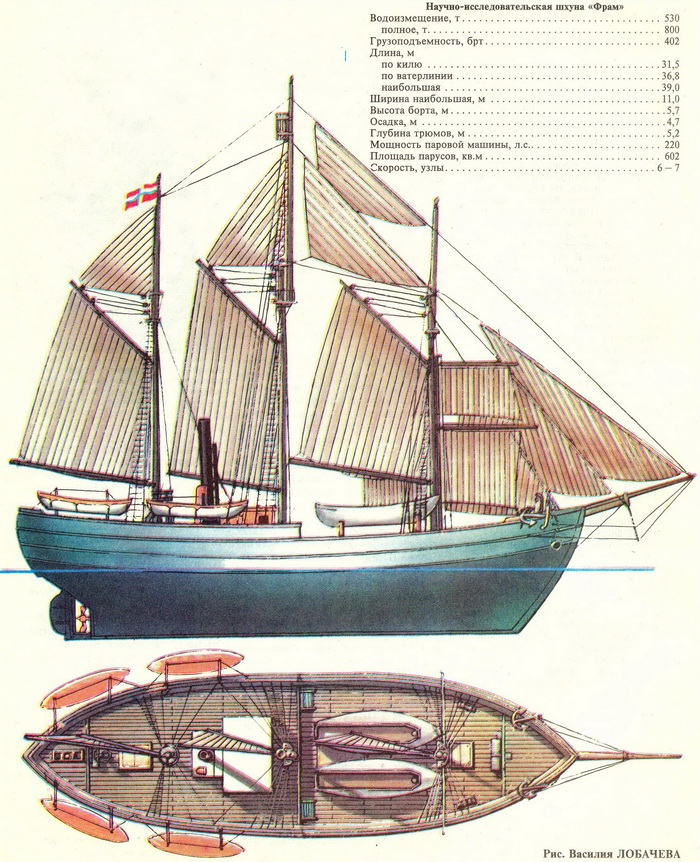
\includegraphics[width=1\textwidth]{Figs/FRAM.jpg}
    \caption{Исследовательское судно <<Фрам>>}
    \label{fig:fram}
\end{figure}

\begin{figure}
    \centering
    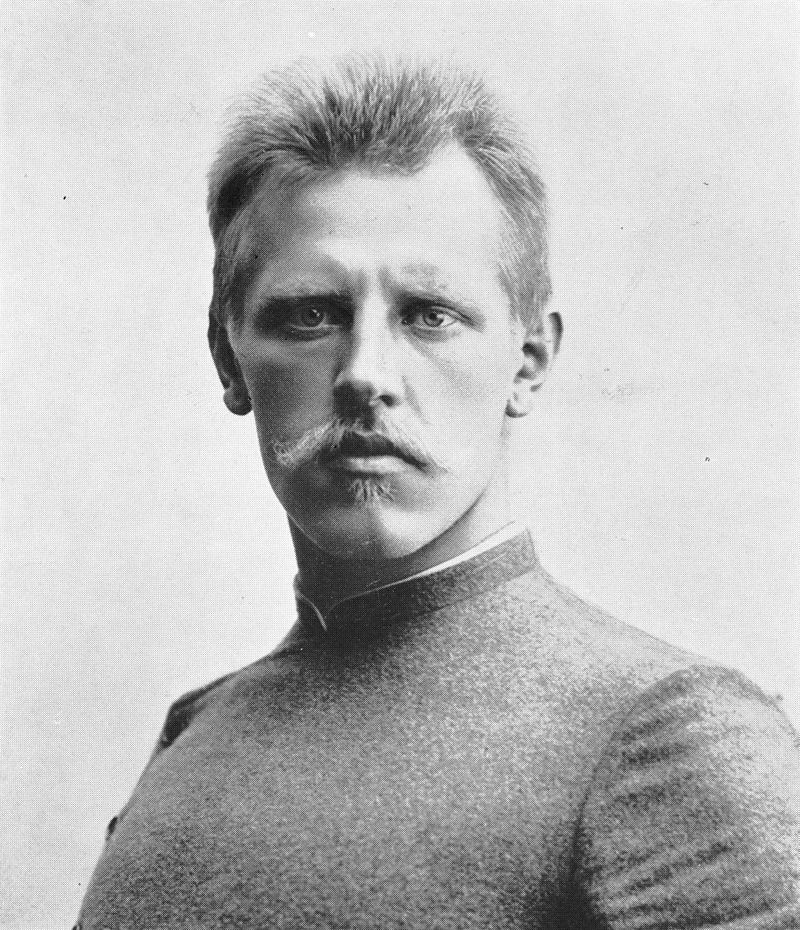
\includegraphics[scale=2.5]{Figs/800px-Fridtjof_Nansen.jpg}
    \caption{Фритьоф Ведель-Ярлсберг Нансен (1861-1930)}
    \label{fig:Nansen}
\end{figure}

Однажды во время штиля судно остановилось. Скорость его движения резко снизилась.  «Чтобы пройти то небольшое расстояние, которое мы и на веслах прошли бы в полчаса или того меньше, «Фраму» понадобилась целая вахта», -- как писал сам Нансен. При этом исследователь отмечал, что вода на поверхности была пресной, потому как натекла с оттаявших ледников. А на глубине сравнимой с осадкой судна, резко становилась соленой. Позднее его записи послужили стимулом для теоретических исследований этого явления. В итоге было установлено, что почти вся энергия судового двигателя сдвигает не судно, а образует волны на поверхности раздела между слоями пресной и соленой воды. Это явление получило название <<мертвая вода>>.

Также существует еще одно свидетельство этого явления. Теплоход «Маршал Жуков» при проходе пролива Дарданеллы угодил в <<мертвую воду>> летом 1981 года. Уже в сентябре в отраслевой газете <<черноморец>> капитан-наставник Александр Косилов подробно описал как в течение четырех суток судно, держащее курс из Канады в Новороссийск, боролось с феноменом. Согласно комментариям руководителя аналитико-исследовательской группы управления инвестиций и проектов ОАО «Новошип», кандидата технических наук, профессора кафедры судовождения ГМУ им. адмирала Ф.Ф. Ушакова Юрия Пескова современные суда в значительной степени подвержены влиянию подобных явлений\cite{MorVest}. На то есть причины:

\begin{itemize}
    \item Экономия топлива вынуждает снижать скоростные режимы
    \item Борьба за уменьшение углекислых выбросов предписывает снижать мощность двигателя
\end{itemize}


\begin{figure}
    \centering
    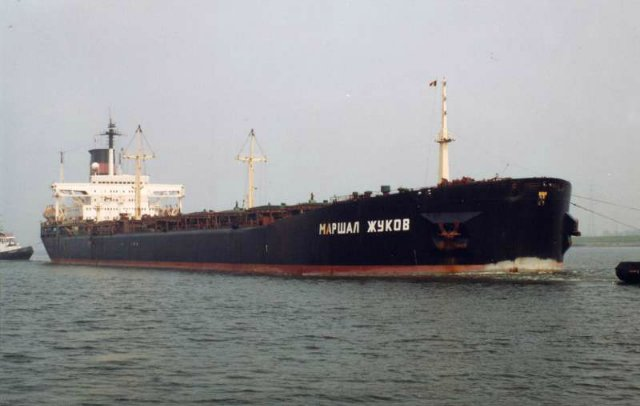
\includegraphics[scale=0.5]{Figs/marshl_jukov.jpg}
    \caption{Судно <<Маршал Жуков>>}
    \label{fig:jukov}
\end{figure}

И подобные явления, как оказалось, описывались и задолго до Франклина. В своей <<естественной истории>> Плиний Старший говорит о похожем явлении \cite{Plinii}. Позднее <<мертвая вода>> была воспроизведена в лабораторных условиях исследователями из франции \cite{deadWater}. Запись эксперимента доступна на видеохостинге youtube \cite{deadWaterVideo}.

О возможности внутренних волн многократно фокусироваться после отражения от наклонных поверхностей стало известно сравнительно недавно \cite{Gardner1989}. Благодаря этому в стратифицированной жидкости могут образовываться аттракторы внутренних волн -- замкнутые траектории по которым циркулируют внутренние волны \cite{Maas1995}.

Внутренние волны активно взаимодействуют с другими океаническими явлениями \cite{Rainville2006} и с неровностями океанического дна \cite{DAUXOIS1999}. Процессы перемещения внутренних волн их взаимодействия друг с другом и океаническими структурами различных масштабов образуют собой явление называемое энергетическим каскадом \cite{Garrett1972}. Энергетический каскад способствует поддержанию глобальной океанической циркуляции и перемешиванию \cite{Nikurashin2012,Munk1998}. Тем не менее, механизмы вносящие крупномасштабный приливный вклад в движение внутренних волн недостаточно понятны \cite{Ivey2008,Polzin1997} и каскадный процесс остается одной из фундаментальных проблем современной океанографии. Главным образом остаются вопросы связи крупномасштабных и мелкомасштабных явлений.

Одним из объяснений этой связи могут послужить аттракторы внутренних гравитационных волн. Это явление, при котором внутренние волны многократно отражаясь от поверхности океана, его дна и неровностей движутся по замкнутым орбитам. Возникновение такого явления возможно лишь в том случае, когда на дне океана имеются определенные комбинации геометрических неровностей. Аттракторы передают кинетическую энергию крупномасштабных эффектов, такие как приливы и внутренние волны большой длинны к мелкомасштабным явлениям волновой турбулентности и перемешиванию. Происходит это благодаря явлению фокусировки, в результате которого длинна внутренних волн уменьшается, но увеличивается амплитуда.

Возможность возникновения аттракторов в океане с реальной геометрией дна уже исследовалась\cite{Tang2010}. Например, топология северной части хребта Лусона имеет соответствующую геометрию. Эксперименты~\cite{ECHEVERRI2011} подтверждают возможность образования аттракторов внутренних волн. Кроме того при моделировании внутренних волн в условиях случайного разреза геометрии океанического дна, был сделан вывод, что с немалой вероятностью возможны возникновения аттракторов по одному на каждую сотню километров океанического дна \cite{Guo2015}. Тем не менее стоит отметить, что на данный момент нет свидетельств наблюдаемых волновых аттракторов. Возможно это связано с тем, что теоретические работы \cite{Guo2015} относятся к двумерному океану, но также существуют трехмерные конфигурации геометрий в которых возможны существования трехмерных волновых аттракторов \cite{Drijfhout2007,Manders2004}. Кроме того, в теоретическом представлении аттракторов внутренних волн не учитывается шероховатость поверхностей отражения. Однако надежность теоретических соображений о возможности существования трехмерных аттракторов была экспериментально проверена \cite{Hazewinkel2010}. Кроме того волновые явления в океане часто имеют целый спектр частот \cite{Garrett1972}, в то время как многочисленные эксперименты проводятся лишь с монохроматическим источником внутренних волн.

Предполагается, что аттракторы могут влиять не только на перемешивание, но и на движение мелких животных, явление седиментации и эрозию прибрежных конструкций.

Работы по фокусировке внутренних волн и образованию устойчивых аттракторов ведутся с конца двадцатого века. Первое теоретическое предсказание аттракторов было сделано Лео Маасом в 1995 году\cite{Maas1995}. Через два года последовали экспериментальные исследования этого явления, теоретические результаты были воспроизведены\cite{Maas1997}. Эффекты фокусировки характерны не только для стратифицированной жидкости, но и для вращающихся \cite{articleMaas2003,Veronis1970}. В дальнейшем теоретические основы явления были пересмотрены на основании данных эксперимента\cite{Lam2008}.

Вместе с развитием вычислительной техники развивались и инструменты численного моделирования физических явлений. Во втором десятилетии двадцать первого века стало возможным численное моделирование трехмерных аттракторов внутренних волн. Первая удачная попытка была предпринята с использованием метода спектральных элементов \cite{Brouzet2016,Brouzet_2016}. При сравнении с экспериментом ошибка численного моделирования составила не более 10\%. Помимо этого аттракторы внутренних волн моделировались с помощью метода конечного объема \cite{Brouzet2014}. Количественно воспроизвести результаты, полученные с помощью метода спектральных элементов не удалось.
Традиционно для моделирования аттракторов применяются уравнения Навье-Стокса в приближении Буссинеска. Однако существует ряд работ, где вместо классического подхода используется квазигидродинамический \cite{ElizarBook}. Квазигидродинамические уравнения позволяют добиться большей точности \cite{Kraposhin20182} при моделировании методом конечного объема.



\section{Общая теория внутренних гравитационных волн}

\subsection{Стратификация}

\begin{figure}
    \centering
    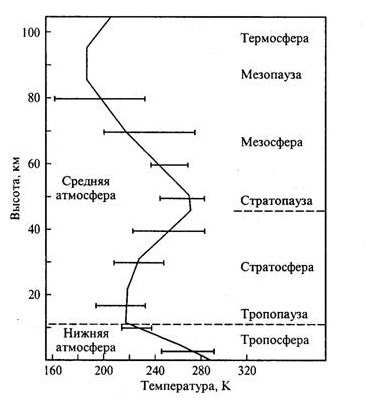
\includegraphics{pics/tempDistrib.jpg}
    \caption{Распределение температуры в атмосфере по высоте}
    \label{fig:temperatureDistrib}
\end{figure}

Рисунок \ref{fig:temperatureDistrib} из \cite{geoThermins} показывает типичное распределение температуры воздуха по высоте. Стратификация в атмосфере измеряется с помощью метеозондов. Выделяются различные регионы с примерно постоянным градиентом температуры: тропосферу, стратосферу, мезосферу и термосферу \cite{saha2008the}. Границы между этими зонами называют тропопауза, стратопауза и мезопауза. Температурный профиль не монотонен, но плотность атмосферы зависит от температуры и давления, которые значительно меняются с высотой. Например, от земли (Высота $= 0$ км.) до стратопаузы (Высота $= 50$ км.), давление уменьшается на три порядка и на шесть до верхних слоев атмосферы (Высота $= 100$ км.). Для этого вводится понятие потенциальной температуры, которая измеряется при одинаковом давлении \cite{gidrometDict}.  Частота плавучести в атмосфере составляет порядка $10^{-2}$ 1/с. 

Океан стратифицирован по солености, как это показано на рис \ref{fig:salVSdepth}. Стратификация зависит от географического положения. Однако можно выделить три основных типа слоев:

\begin{itemize}
    \item Смешанный слой, расположенный несколько ниже поверхности. Этот слой имеет толщину около $100$ м и однороден по температуре и солености. Перемешивание происходит из-за различных взаимодействий с атмосферой. 
    
    \item Область ниже смешанного слоя. В этой области плотность изменяется квазилинейно с глубиной на несколько километров. Частота плавучести в этом слое обычно составляет $10^{-4}$ --- $10^{-3}$ рад/с.
    
    \item Пикноклин, где плотность резко меняется. Этот слой очень тонкий и расположен между смешанным слоем и глубинной областью. Таким образом, он демонстрирует сильные градиенты плотности, а частота плавучести в этом слое обычно составляет $10^{-2}$ рад/с. Пикноклин ограничивает обмены между смешанным слоем и глубинной областью из-за сильных градиентов плотности.
\end{itemize}


\begin{figure}
    \centering
    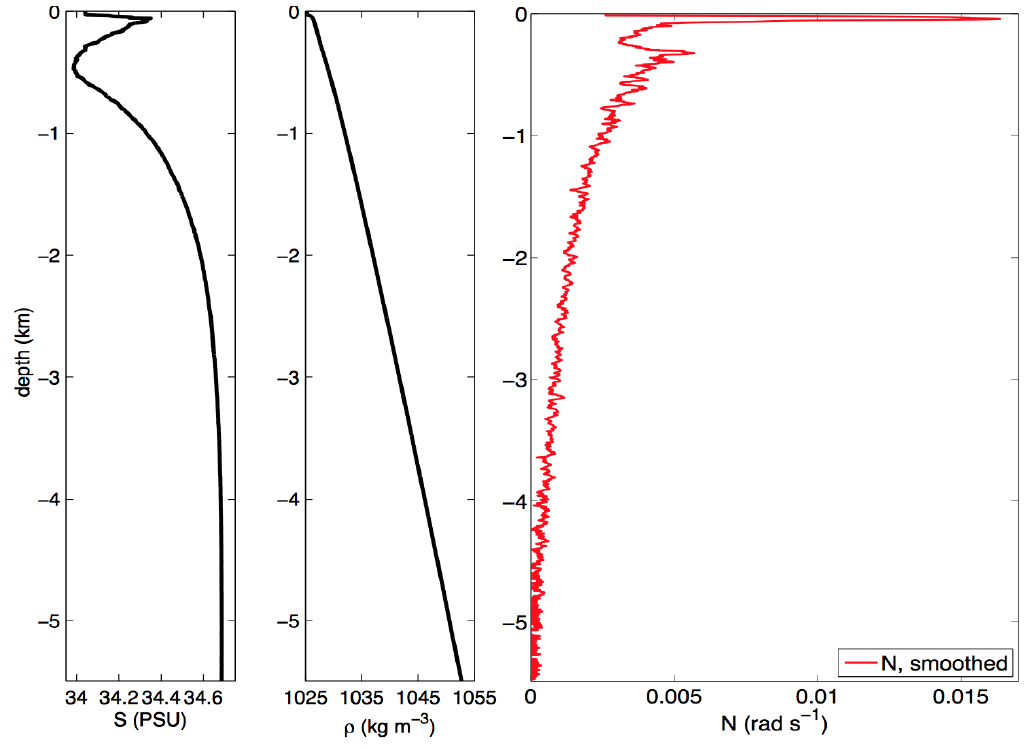
\includegraphics[scale = 0.6]{pics/salinityAndNVsDepth.png}
    \caption{Распределение солености, плотности и частоты плавучести в океане по глубине}
    \label{fig:salVSdepth}
\end{figure}

\subsection{Генерация внутренних волн}

В атмосфере внутренние волны рождаются от взаимодействия ветров и рельефа земной поверхности.

В океане есть два механизма ответственных за происхождение внутренних волн:

\begin{itemize}
    \item Излучение внутренних волн топографией морского дна во время приливных течений. К примеру обтекание приливным потоком топологической возвышенности высотой 100 м при частоте плавучести $10^{-3}$ рад/приведет к возникновению внутренних волн если скорость потока превышает $0.4$ м/с. Рисунок \ref{fig:intWaveGen} из \cite{GarrettSc} показывает как приливное воздействие генерирует внутренние волны. Также от взаимодействия с шельфом, как показано в левой части рисунка \ref{fig:intWaveGen}
    \item Из-за взаимодействия с атмосферой посредством ветра. 
\end{itemize}

\begin{figure}
    \centering
    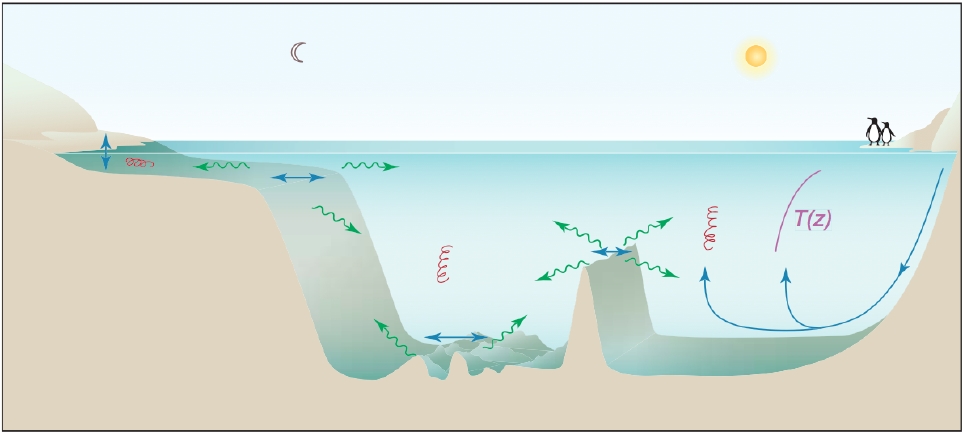
\includegraphics[scale=0.6]{pics/IntGen.png}
    \caption{Генерация внутренних волн за счет приливного воздействия \cite{GarrettSc}. В центре волны вызваны приливами. Слева волны вызваны приливами вблизи континентального шельфа. Волны способствуют возникновению турбулентности, и перемешиванию в океане, влияют на профиль плотности, как показано справа.}
    \label{fig:intWaveGen}
\end{figure}

Внутренние волны могут вызывать перемешивание в океане и играть существенную роль в океанографической циркуляции. Вертикальное перемешивание в стратифицированной жидкости имеет первостепенное значение для глобального обращения. В около 90\% из примерно 60 ТВт мощности, поступающей от ветра в океан, рассеивается в пределах 100 м от поверхности воды \cite{Ferrari2009} за счет волновой турбулентности \cite{nazarenko2011wave, Yarom2014} и опрокидывания внутренних волн \cite{Perlin2013}. Механизм перемешивания при больших глубинах менее изученное явление. Океанографические данные говорят о том, что для поддержания имеющийся стратификации необходимо 1 ТВт мощности \cite{Munk1998}. Постоянное воздействие приливных эффектов на океан имеет мощность порядка 11 ТВт \cite{Garrett2007}. Поэтому должен существовать механизм конвертации (так называемый энергетический каскад) мощности поступающей со стороны приливных эффектов в многообразие внутренних волн различных масштабов и перемешиванию \cite{Munk1998}.

Причем нет единой точки зрения на то какие механизмы перемешивания в глубинных слоях океана являются доминирующими \cite{Ivey2008}. Существуют описания составляющих энергетического каскада, фокусировка внутренних волн \cite{BHLER2007}, отражение внутренних волн \cite{dauxois_young_1999}, преломление волн в слоях с резким перепадом плотности \cite{mathur_peacock_2009}, интерференция волн и их взаимодействие со сложной топографией морского дна \cite{ECHEVERRI2011}, внутренние волны Ли \cite{MacKinnon2013,Nikurashin2013}. Допускаются сценарии с триадной резонансной неустойчивостью \cite{Bourget2013}, гидростатической неустойчивостью \cite{mathur_peacock_2009}, сдвиговой неустойчивостью и неустойчивостью нижнего слоя на склонах \cite{Gayen2010, Lamb2014}.

Математически описать возникновение внутренних волн можно записав уравнение для сил, которые действуют на выведенную из равновесия частицу жидкости(Рис. \ref{fig:Forces}):

\begin{figure}
    \centering
    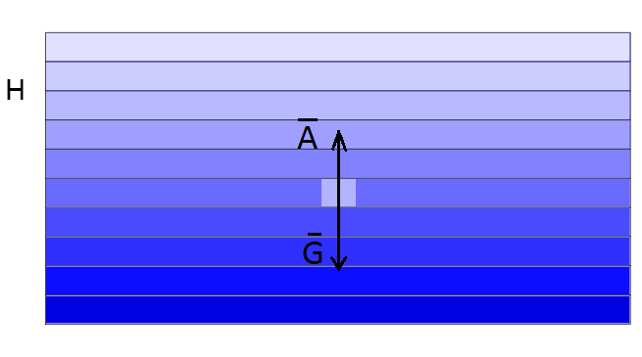
\includegraphics[scale=0.8]{Figs/Forces.png}
    \caption{Схематичное представление сил действующие на частицу выведенную из равновесия в стратифицированной жидкости, цветом показана плотность.}
    \label{fig:Forces}
\end{figure}

\begin{equation}
    m_b \vec{a}_b = \vec{P} + \vec{G}
\end{equation}
где $\vec{P}=\rho_w \vec{g} S \cdot h$ это сила Архимеда, $\rho_w$ плотность жидкости того слоя на котором находится частица, $\vec{g}$ -- ускорение свободного падения, $S$ -- площадь стороны частицы, $h$  -- глубина. $\vec{G} = \rho_b \vec{g} S \cdot h$,  $\rho_b$ -- плотность частицы жидкости.

В проекции на вертикальную ось:

\begin{equation}
    \frac{d^2 \xi}{dt^2} = \frac{(\rho_w-\rho_b)}{\rho_b}\cdot g
\end{equation}

Тут $\xi$ будет обозначать отклонение от положения равновесия $z_0$, тогда очевидно что плотность воды вокруг частицы и плотность частицы будет равна в положении равновесия при $\xi=0$ $\rho_w(z_0)=\rho_b$ тогда уравнение можно переписать:

\begin{equation}
    \frac{d^2 \xi}{dt^2} = \frac{\rho_w(z_0+\xi)-\rho_b}{\rho_b}\cdot g
    \label{eq:beg}
\end{equation}

Введем переобозначение, $z=z_0+\xi$ тогда правая часть уравнения запишется $$\frac{\rho_w(z_0+\xi)-\rho_b}{\rho_b}\cdot g = \frac{\rho_w(z)-\rho_w(z_0)}{\rho_w(z_0)}\cdot g = \frac{1}{\rho(z_0)} \frac{\rho_w(z)-\rho_w(z_0)}{z-z_0}\cdot(z-z_0) g$$

При достаточно малом $t$ отклонении от положения равновесия $z$ будет также мало, что дает нам возможность перейти к производной по $z$, а $\rho_w$ переобозначим как $\rho$ и окончательно запишем:

\begin{equation}
    \frac{d^2 \xi}{dt^2} =\frac{1}{\rho} \frac{d\rho}{z}\xi \cdot g
\end{equation}

Решение этого дифференциального уравнения ищется в виде периодической функции, это значит, что частица совершает колебания около своего положения равновесия:

\begin{equation}
    \xi(t)=A cos(\omega t + \phi)
\end{equation}

подставим выражения $\xi(t)$ в уравнение:

\begin{equation}
    \ddot{\xi} = - A \omega^2 cos(\omega t + \phi )
\end{equation}

или если выразить правую часть через $\xi$

\begin{equation}
    \ddot{\xi} = - \omega^2  \xi
    \label{eq:final}
\end{equation}

Подставим (\ref{eq:final}) в (\ref{eq:beg}):

\begin{equation}
    -\omega^2 \xi = \frac{1}{\rho_0}\cdot \frac{d \rho}{d z} \xi g
\end{equation}

Выразим частоту колебаний частицы:

\begin{equation}
    \omega(z) = N(z) = \sqrt{- \frac{g}{\rho_0}\cdot\frac{d \rho(z)}{dz}}
\end{equation}

Эта частота называется частота плавучести или Частота Брента — Вяйсяля. В океане она составляет величину порядка $10^{-3}$ $\frac{1}{\textup{с}}$ \cite{King2012}.


\subsection{Математические модели для изучения внутренних гравитационных волн}

Для описания движения несжимаемой жидкости используется уравнение Навье-Стокста. Но при небольшом перепаде плотности допустимо использовать уравнение Навье-Стокса в приближении Буссинеска, которое учитывает сжимаемость в члене с плавучестью.

\begin{equation}
 \large \frac{\partial \vec U}{\partial t} + (\vec U \cdot \nabla) \vec U = - \frac{1}{\rho_m} \nabla \hat p + \nu \Delta \vec U  + \vec f,
 \label{eq:momClassic}
\end{equation}
Уравнение переноса соли $s$:
\begin{equation}
 \large \frac{\partial \rho_s}{\partial t} + \vec U \cdot \nabla \rho_s  = \nabla \cdot \frac{\nu}{Sc} \left ( \nabla \rho_s \right ),
 \label{eq:transClassic}
\end{equation}
\begin{equation}
 \large \nabla \cdot \vec U  = 0.
 \label{eq:contClassic}
\end{equation}

Здесь $\vec{U}$ -- вектор скорости с компонентами $u_x,u_y; \nu$ -- кинематическая вязкость жидкости; $\rho_m$ -- значение плотности на верхней границе; $\rho_s$ -- добавка к плотности обусловленная наличием солености; приведенное давление $\hat{p}=p-p_0$, разница между полным и гидростатическим давлением; $\vec{f}=\frac{\rho_s}{\rho_m} \vec{g}$ -- восстанавливающая сила; Число Шмидта представляет собой отношение кинематической вязкости и коэффициента диффузии:  $Sc = \frac{\nu}{D}$. 

В данной работе помимо классических уравнений Навье-Стокса в приближении Буссинеска используются квазигидродинамические уравнения, работа над которыми ведется в институте прикладной математики имени Келдыша с восьмидесятых годов двадцатого века \cite{bookELIZ}. Различие между уравнениями Навье-Стокса несжимаемой жидкости и квазигидродинамическими уравнениями заключается в дополнительных диссипативных слагаемых. Эти слагаемые были первоначально введены для разреженного газа как способ сохранить инвариантность при пространственно-временном усреднении\cite{AIAAJ1995}. Физическая интерпретируемость в случае несжимаемой жидкости после обобщения теряется, но математически уравнения все еще верны \cite{Elizarova2011}. Как будет показано ниже диссипативные слагаемые могут быть весьма полезны при численном моделировании. 

\subsection{Линеаризованная теория внутренних гравитационных волн}

Ранее рассмотрена полная система уравнений, описывающая движение стратифицированной жидкости. Чтобы упростить задачу, можно предположить, что поток является двумерным и содержится в плоскости $xOz$ без изменений в направлении $y$. В этих рамках, используя уравнение неразрывности (\ref{eq:contClassic}), можно ввести функцию тока, определяемую как

\begin{equation}
    \frac{\partial \psi}{\partial x} = - u_z \;\;\;\;\;\;\;\; и \;\;\;\;\;\;\;\; \frac{\partial \psi}{\partial z} = - u_x
\end{equation}

тогда можно переписать уравнения (\ref{eq:momClassic}), (\ref{eq:transClassic}) и (\ref{eq:contClassic}) как

\begin{equation}
    \partial_{tz} \psi + J(\partial_z \psi, \psi) = - \frac{1}{\rho} \partial_x P + \nu \partial_z \Delta \psi,
    \label{eq:tokz}
\end{equation}

\begin{equation}
    \partial_{tx} \psi + J(\partial_x \psi, \psi) = \frac{\rho_s}{\rho_m}\vec{g}+\frac{1}{\rho}\partial_z P + \nu \partial_x \Delta \psi,
    \label{eq:tokx}
\end{equation}

\begin{equation}
    \partial_t \rho_s + J(\rho_s,\psi) = \nabla \cdot \frac{\nu}{Sc} (\nabla \rho_s) + \frac{d \rho}{dz} \partial_x \psi,
\end{equation}
где $J$ это якобиан определенный как $J(f,g) = \partial_x f \partial_z g - \partial_z f \partial_x g.$ Обозначим как $\partial_j \psi =\frac{\partial \psi}{\partial j}$, где $j$ обозначает $x,y$ или $t$. 

В дальнейшем предполагается, что возмущения плотности $\rho_s(x; z; t)$ малы по сравнению с фоновой стратификацией $\rho(z)$. Это предположение полностью верно как в океане, так и экспериментах, рассматриваемых тут. Таким образом, возмущения плотности ограничиваются менее чем 10\% средней стратификации. 

Дифференцируя уравнение (\ref{eq:tokz}) по $z$, а (\ref{eq:tokx}) по $x$ и складывая их получаем

\begin{equation}
    \partial_t(\Delta \psi) + J (\Delta \psi, \psi) - \nu \Delta (\Delta \psi) = \frac{g}{\rho_m} \partial_x \rho_s,
    \label{eq:tokzz}
\end{equation}

\begin{equation}
    \partial_t \rho_s + J(\rho_s,\psi) - \nabla \cdot \frac{\nu}{Sc} (\nabla \rho_s) = -N^2 \frac{\rho_m}{g}\partial_x \psi.
    \label{eq:tokxx}
\end{equation}

Уравнения (\ref{eq:tokzz}) и (\ref{eq:tokxx}) описывают нелинейную динамику вязкой стратифицированной жидкости с диффузией. Уравнения для линейной динамики получаются путем пренебрежения нелинейными членами. Это приводит к

\begin{equation}
    \partial_t(\Delta \psi) + \nu \Delta (\Delta \psi) = \frac{g}{\rho_m} \partial_x \rho_s,
\end{equation}

\begin{equation}
    \partial_t \rho_s - \nabla \cdot \frac{\nu}{Sc} (\nabla \rho_s) = -N^2 \frac{\rho_m}{g}\partial_x \psi.
\end{equation}

Рассмотрим решение в виде плоской волны к линеаризованной системе: $\psi = \psi_0 exp(i\omega t - i \vec{k} \cdot \vec{r})$ и $\rho_s=\rho_m exp(i\omega t - i \vec{k}\cdot \vec{r})$. Волновой вектор $\vec{k}=k_x \vec{e}_x + k_z \vec{e}_z$ и его модуль $k$.

Линейная система может быть записана в матричном виде

\begin{equation}
    \left(\begin{array}{cc} -k^2(i\omega + \nu k^2) & i \frac{g}{\rho_m}k_x
    \\[15pt] iN^2 \frac{\rho_m}{g}kx & i\omega + \frac{\nu}{Sc} k^2 \end{array}\right)
    \left(\begin{array}{c}\psi \\[15pt] \rho_s\end{array}\right) = 
    \left(\begin{array}{c}0 \\[15pt] 0\end{array}\right).
\end{equation}

Можно найти нетривиальное решение этой системы

\begin{equation}
    k^2 \left( i\omega + \nu k^2 \right) \left(i \omega \frac{\nu}{Sc} k^2 \right) + N^2 k^2_x = 0.
\end{equation}

Если рассмотреть систему без диссипативных членов, убрать диффузию и теплопроводность то уравнение примет вид:

\begin{equation}
    \left(\frac{\omega}{N}\right)=\frac{k^2_x}{k^2} \;\;\;\;\;\;\;\; или \;\;\;\;\;\;\;\; \frac{\omega}{N}=\pm \frac{|k_x|}{k}.
\end{equation}

Это дисперсионное соотношение линейных внутренних волн в невязкой и недиффузионной жидкости. Его можно записать, используя угол $\theta$ между вертикальной осью $z$ и волновым вектором $\vec{k}$

\begin{equation}
    \frac{\omega}{N} = \pm sin \theta.
    \label{eq:dispersion}
\end{equation}

Это чисто геометрическое соотношение, которое показывает как распространяются волны в стратифицированной жидкости(Рис. \ref{fig:ermExp}). Угол распространения определяется только частотой плавучести и частотой вынужденных колебаний. Наконец, стоит отметить, что в дисперсионном соотношении отсутствует характерный масштаб длины. Таким образом, длина внутренних волн определяется граничными условиями, только источником волн.

\begin{figure}
    \centering
    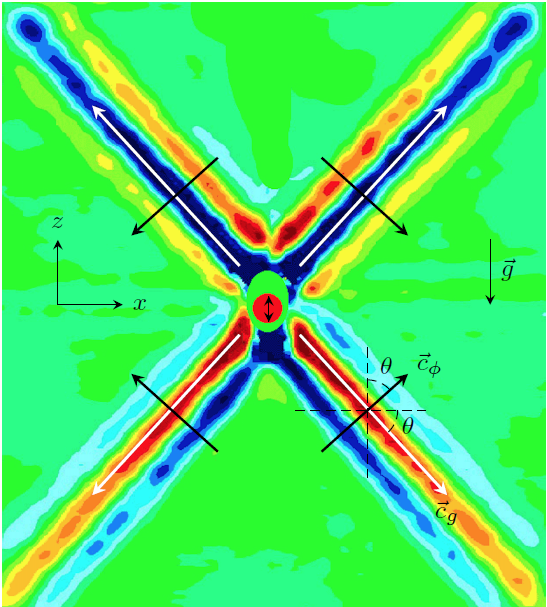
\includegraphics[scale=0.5]{Figs/Experement_Erm.png}
    \caption{Внутренние волны, излучаемые вертикально колеблющимся цилиндром, распространяются в линейно стратифицированной жидкости и  показаны красным в центре рисунка. Векторы групповой скорости показаны белым цветом, а векторы фазовой скорости — черным. Цветами обозначены поля горизонтального градиента плотности, полученные экспериментально Евгением Ерманюком с использованием методики SyS. Рисунок из \cite{brouzet:tel-01361201}}
    \label{fig:ermExp}
\end{figure}

%\subsection{Численные методы исследования волновых течений в неоднородных средах}

\section{Аттракторы внутренних волн}

Первые работы по аттракторам внутренних волн были проведены Лео Маасом, сначала теоретические \cite{Maas1995}, а потом и экспериментальные \cite{brouzet1997laboratory}.  

Дисперсионное соотношение дает мощный инструмент позволяющий качественно предсказать траекторию движения пучков внутренних волн, не только по удалению от источника, но и при отражении от препятствий (Рис. \ref{fig:internalReflection}). Поле отражения внутренняя волна сохраняет угол с вертикалью. Кроме того внутренние волны обладают свойством фокусировки, что выражается в сокращении расстояния между двумя параллельно пущенными лучами поле отражения от наклонной стенки. 

\begin{figure}
    \centering
    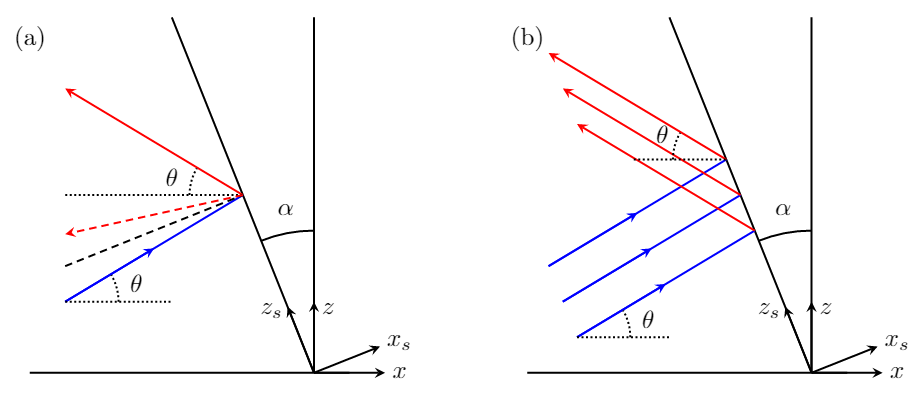
\includegraphics[scale=0.5]{Figs/angle_of_reflection.png}
    \caption{Отражение пучка внутренних волн от наклонной стенки. а) Отражение одного пучка, падающий волновой луч изображен синим цветом, отраженный от наклонной стенки красным, точками обозначена биссектриса. Черным пунктиром обозначен перпендикуляр к наклонной поверхности, красным пунктиром луч отраженный <<зеркально>> по правилу Евклида. b) Отражение нескольких волновых лучшей от наклонной поверхности, отраженные лучи стали ближе, чем были падающие.}
    \label{fig:internalReflection}
\end{figure}

Многократное отражение от стенок трапециевидного резервуара приведет к постепенному сближению лучей, которые, в конечном итоге замкнуться на траектории в форме параллелепипеда (Рис. \ref{fig:RayTr}). 

\begin{figure}
    \centering
    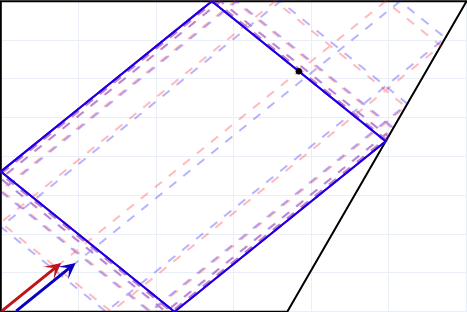
\includegraphics[scale=0.8]{Figs/RayTracing.png}
    \caption{Результат многократного отражения двух параллельных лучей внутренних волн}
    \label{fig:RayTr}
\end{figure}



\subsection*{Заключение к главе 1}

Явление внутренних волн широко распространенное в океане оказывает огромное влияние на природные процессы происходящих в его недрах, на климатические процессы в атмосфере, а также на жизнедеятельность человека. 

В этой главе рассматривается история открытия и развития теории внутренних волн, переломным моментом в исследовании явлений связанных с динамикой стратифицированной жидкости можно считать экспедицию Нансена. Проведен обзор литературы по теме внутренних гравитационных волн, благодаря специальному закону отражения от наклонных поверхностей, который определяется дисперсионным соотношением у внутренних волн имеется свойство фокусировки. Фокусировка позволяет внутренним волнам образовывать аттракторы внутренних волн в закрытых акваториях. В главе рассмотрены геометрические и физические принципы фокусировки. 